\documentclass{article}
\usepackage{amsmath}
\usepackage{amssymb}
\usepackage{hyperref}
\usepackage{graphicx}
\usepackage{natbib}
\usepackage{booktabs}
\graphicspath{ {./data/results} }

\title{K-NN Based Prior for Option Pricing Strategy}
\author{Ayan Goswami}
\date{}
\begin{document}
\maketitle
\section{Abstract}

We present a non-parametric framework for modeling and trading short-term equity options using K-Nearest Neighbors (KNN) trying to estimate the prior distribution of option price. By predicting standardized option prices from key Greeks and volatility measures, we identify residuals with predictive power for future returns. A directional hypothesis test confirms that under- and over-predicted options exhibit statistically significant forward price behavior. A simulated trading strategy using residual-based signals outperforms randomized baselines with strong significance. This work demonstrates a pragmatic use of estimation, providing evidence for short-term inefficiencies in option markets.

\section{Introduction}

This document summarizes the findings reported in \texttt{strategy\_book.pdf}. The original analysis uses option data to evaluate pricing efficiency and develop a trading approach. Short-dated options have become increasingly popular in modern markets, yet pricing them efficiently remains a challenge. Traditional models such as Black-Scholes assume constant volatility and smooth dynamics, often invalid in practice. We adopt a K-Nearest Neighbors regression model to estimate standardized option prices, bypassing strong parametric assumptions.

\section{Methodology}

Our approach has three key components: (i) exploratory analysis of option features, (ii) KNN-based prediction of standardized prices using Greeks and moneyness, and (iii) residual-based hypothesis testing to detect mispricings that yield directional signals for trading.

\subsection{Data Loading and Preparation}

Option data was loaded from a socket stream leveraging Alpaca's IEX market data, updated every 10 seconds. For the purposes of this investigation, we focused on options with 0 days to expiry (0dte), as they have the largest trading volume and are hence assumed to self-correct quicker than options with a later expiry. All options with strikes between 99\% to 101\% of the current price were stored in a csv, along with all the corresponding greeks and implied volatility. To read more about how this was calculated see the Appendix. When this investigation was conducted, SPY hovered around 620\$, hence for a given timestamp, 14 or 15 calls and puts were stored. This was done to get an even spread of in the money (ITM), at the money (ATM) and out the money (OTM) options.

Moneyness, defined as the relative position of the underlying asset price to the strike price, exhibits a strong relationship with the option premium. For call options, those that are in the money (ITM), i.e., with strike prices lower than the spot price (\(K < S\)), tend to have higher intrinsic value and thus higher premiums. Conversely, out of the money (OTM) options (\(K > S\)) carry mostly time value and are priced lower. This nonlinear relationship is especially pronounced in short-dated options, where the time decay is steep and the implied volatility surface varies across moneyness levels.

There is usually a very steep drop-off in 0dte OTM options' prices, mainly due to the fact that they will expire worthless by the end of the day. To enable fair comparison of option prices across different timestamps and mitigate scale differences between call and put options, we applied a logarithmic normalization procedure to standardize the prices. The transformation is defined as:

\[
\text{standardized\_price} = \frac{\log(p + 1) - \log(p_{\min} + 1)}{\log(p_{\max} + 1) - \log(p_{\min} + 1)}
\]

where \(p\) is the latest trade price of the option, and \(p_{\min}, p_{\max}\) are the minimum and maximum trade prices for a given option type (call or put) within a specific timestamp. For example, at the first timestamp of the data set: 2025-07-08 08:45:38 (UTC-04:00), with \(p_{\max} = 6.31\) and \(p_{\min} = 0.04\), a call option with strike = 619 and price \(p = 2.71\) would have a standardized price of:

\begin{align}
\text{standardized\_price} &= \frac{\log(2.71 + 1) - \log(0.04 + 1)}{\log(6.31 + 1) - \log(0.04 + 1)} \nonumber \\
&= \frac{\log(3.71) - \log(1.04)}{\log(7.31) - \log(1.04)} \nonumber \\
&= \frac{1.312 - 0.039}{1.989 - 0.039} = \frac{1.273}{1.950} = 0.653
\end{align}

This way, all options at a given timestamp are contextualized, as the options must be analyzed in context of others to determine over/under valued prices. This transformation is applied separately for call and put options, and performed independently at each timestamp. The rationale is twofold: (1) call and put options have inherently different pricing distributions, and (2) the market conditions change across timestamps, requiring local normalization to preserve intra-timestamp price structure. 

Logarithmic scaling was chosen to compress the skewness in price distribution, especially in deep ITM or OTM options where price differences can be exponential. Adding 1 inside the logarithm avoids issues with near-zero prices. The result is a normalized feature \texttt{standardized\_price} bounded in \([0, 1]\), suitable for downstream tasks such as KNN modeling and residual analysis. The following is a random timestamp slice:
\begin{figure}[h]
  \centering
  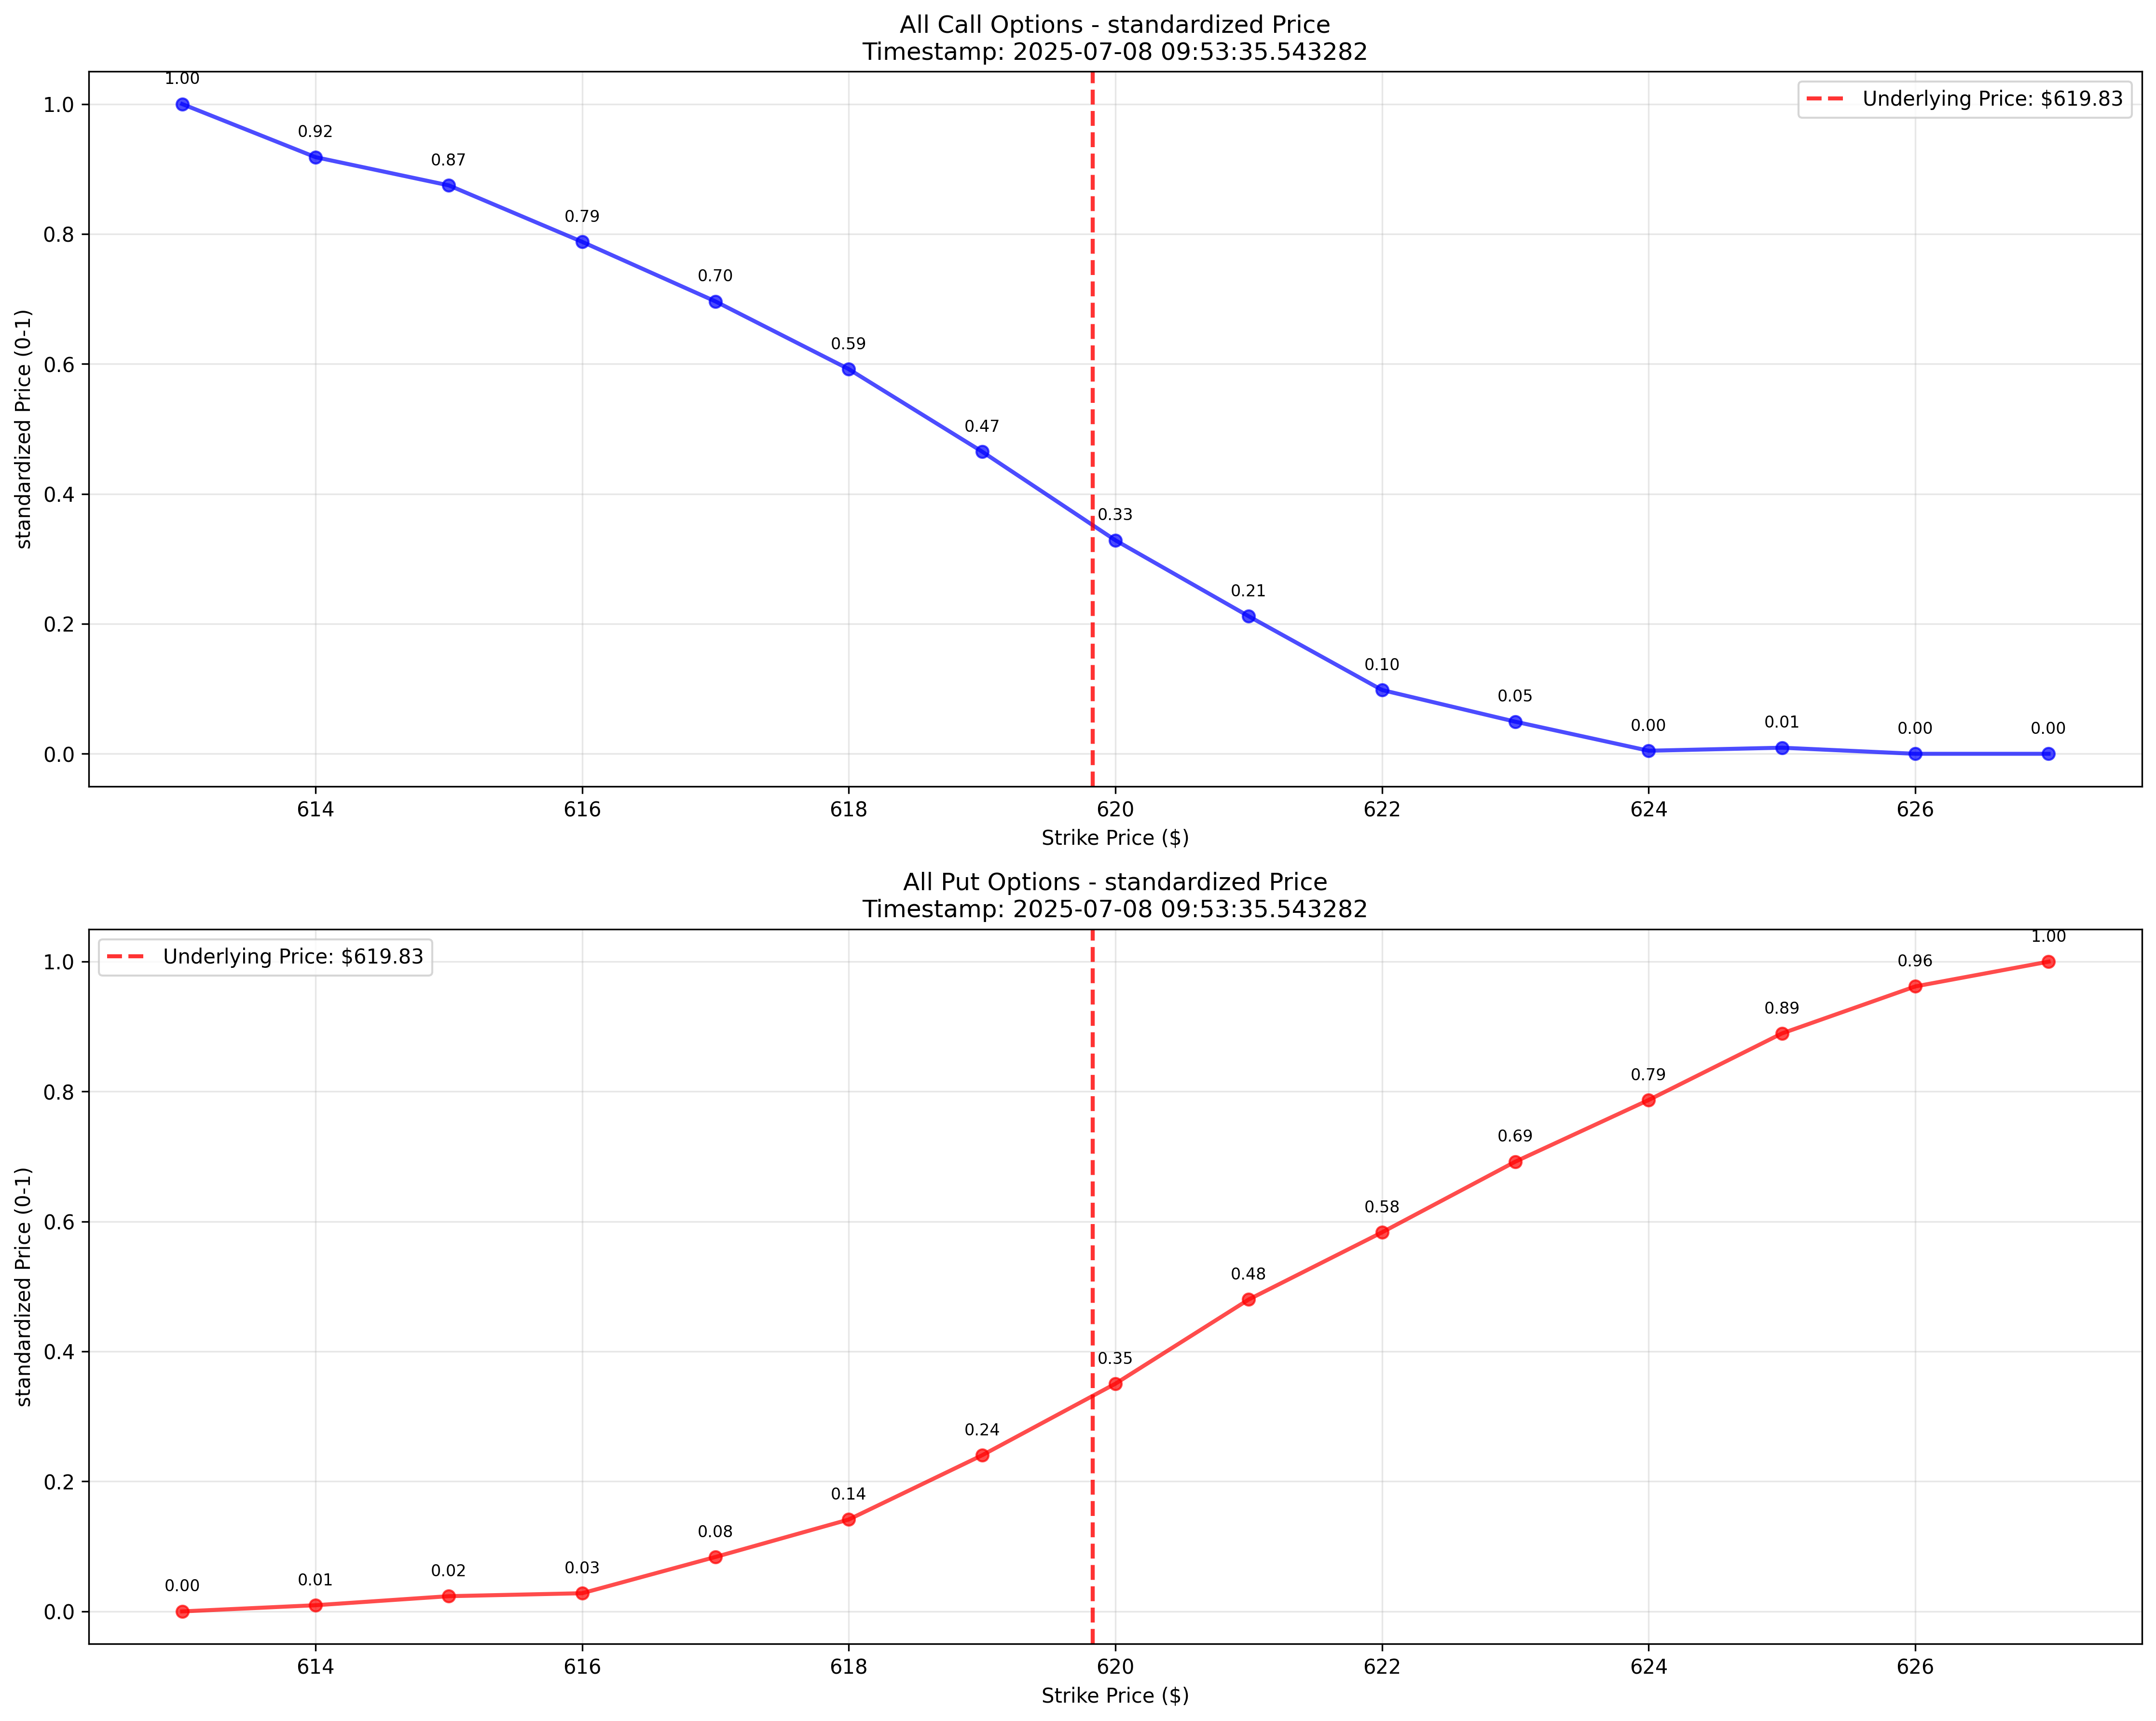
\includegraphics[width=1\linewidth]{calls_puts_timestamp_329}
  \caption{Standardized option prices for a given strike}
  \label{fig:price-std}
\end{figure}

Option data were loaded from several processed files and split into training and validation sets using a 56\%/14\%/30\% split for training, validation and testing. 
Since the $\theta$ decay is so high for 0dte options, we focused on trade entry and exit windows between 30 seconds to 5 minutes. This way the $\alpha$ can be measured reliably without accounting for price decay. Hence, a column was appended to our dataset called \texttt{price\_diff}, which measured:

\[
\text{price\_diff}_x = \frac{\frac{1}{x}\sum_{i=t}^{t+x-1}\text{price}_i}{\text{price}_t}
\]

where x is the look-forward period in tens of seconds, and t is the current time period. This will serve as a metric of success and efficacy in our paper. The top and bottom 5\% were trimmed in this data set to mitigate the risk of outlier-driven distortion in both the residual distribution and downstream performance metrics, such as the estimated significance of prediction errors.

\subsection{KNN Modeling}

K-Nearest Neighbors (KNN) is a non-parametric regression algorithm that predicts the output of a data point based on the average of its $k$ nearest neighbors in the feature space \cite{cover1967nearest}. Unlike parametric models, KNN does not assume a functional form for the relationship between input variables and the target. Instead, it leverages local structure in the data to make predictions. This makes KNN particularly useful in financial contexts where relationships between variables may be complex, noisy, or nonlinear \cite{altman1992introduction}. Our model predicts standardized option prices based on option greeks, volatility and moneyness (see Appendix). A wrapper function scales predictors and returns both root mean squared error (RMSE) and $R^2$ values. Exhaustive subset selection determined that \verb|delta|, \verb|gamma|, \verb|moneyness|, and \verb|rho| gave the best performance with RMSE 0.0269 and \( R^2 = 0.9946 \). The $k$ value used in the analysis was $\sqrt{n}$ where $n$ is the number of rows in the training set. This is standard is most analyses We define the KNN estimator:
\[
\hat{y}_t = \frac{1}{k} \sum_{i \in \mathcal{N}_k(x_t)} y_i
\]

where \( \mathcal{N}_k(x_t) \) is the set of \( k \) nearest neighbors of feature vector \( x_t \). \

Optimal $k$ was found by evaluating a range of values and occurred at $k=3$. Such a low $k$ indicates a complex space, and from our analysis it is possible that the optimal $k$ is 1. $k=1$ would require discussion of the bias-variance trade-off; $k=3$ is our compromise in this regard. The following is the performance of the model on the validation data.

\begin{figure}[h]
  \centering
  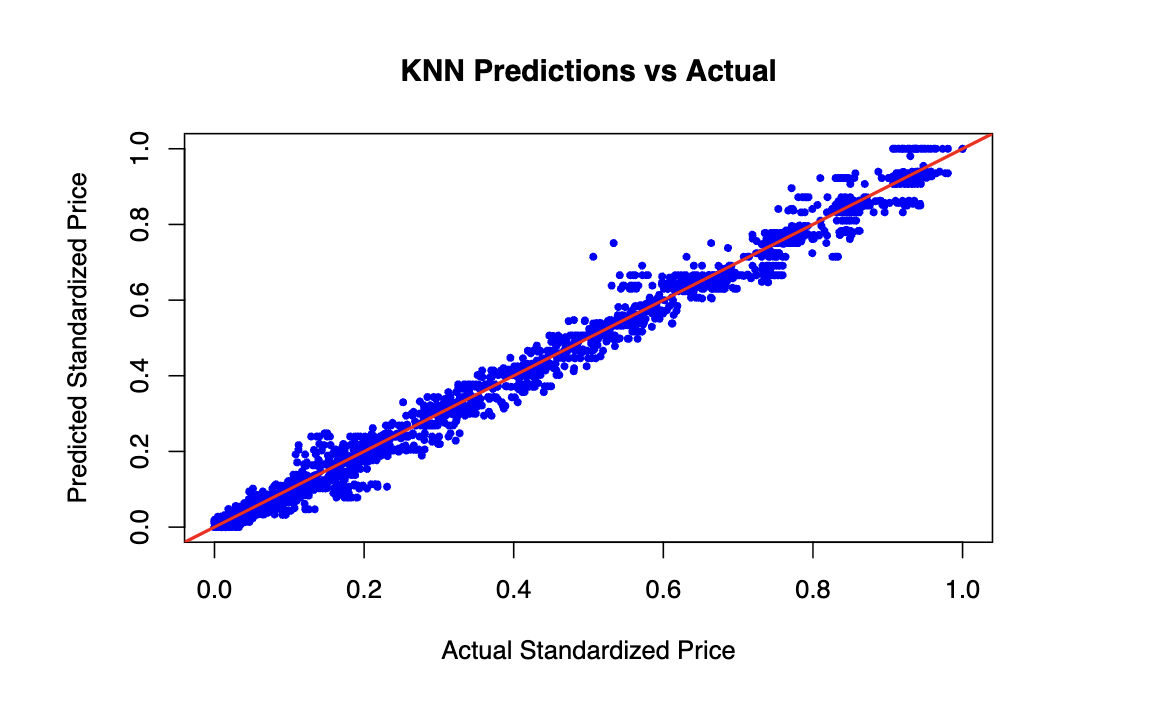
\includegraphics[width=0.8\linewidth]{data/results/knn_preds.png}
  \caption{Predicted vs Actual Standardized prices}
  \label{fig:knn-preds}
\end{figure}

\subsection{Residual Analysis and Hypothesis Testing}

Residuals are defined as:
\[
r_t = \hat{y}_t - y_t
\]
We categorize residuals exceeding the 95th percentile of the empirical distribution as significant. Predictions greater than this threshold $r_t > \bar{r}$ , are interpreted as undervalued options, where the model overestimates the price relative to observed values. Conversely, predictions with residuals below the negative threshold, $r_t < -\bar{r}$, are considered overvalued, where the model underestimates the price. These cases form the basis for directional trading signals. A Shapiro-Wilk normality test revealed a very high confidence that the residuals were normally distributed, hence we were justified in using the same threshold in both cases.
The key hypothesis tested is:
\[
H_1: \mu_{\text{GEQ}} > \mu_{\text{All}} > \mu_{\text{LEQ}}
\]
where \( \mu_{\text{GEQ}} \), \( \mu_{\text{LEQ}} \), and \( \mu_{\text{All}} \) are the mean future price differences ($price\_diff$) for positive, negative, and all residuals, respectively. Directional t-tests were conducted to confirm significance for the time windows.

The null hypothesis was rejected for the 3, 6 and 12 period windows with p-values below 0.05. The alternative hypothesis was partially supported in other horizons. For the purposes of this investigation, we will focus on the 6 period window, as it can provide a more interpretable result which can be extended to shorter and longer time periods. 

\begin{table}[h]
  \centering
  \resizebox{\textwidth}{!}{%
    \begin{tabular}{lcccccc}
      \toprule
      Period (10s) & Mean (Under) & Mean (Over) & Mean (Overall) & $P(\mu_{\text{GEQ}} = \mu_{\text{All}})$ & $P(\mu_{\text{All}} = \mu_{\text{LEQ}})$ \\
      \midrule
      3   & 1.0192 & 0.9912 & 1.0048 & 0.012*  & 0*       \\
      6   & 1.0187 & 0.9885 & 1.0042 & 0.02*  & 0*  \\
      12  & 1.015 & 0.9861 & 1.0033 & 0.045*   & 0*  \\
      15  & 1.014 & 0.9869 & 1.0031 & 0.069   & 0*  \\
      30  & 1.0104 & 0.9899 & 1.0046 & 0.277   & 0.0001*  \\
      \bottomrule
    \end{tabular}%
  }
  \caption{Mean future price ratios by residual group and associated $p$-values. * indicates significance at $p = 0.05$.}
  \label{tab:mean-return}
\end{table}


\begin{figure}[h]
  \centering
  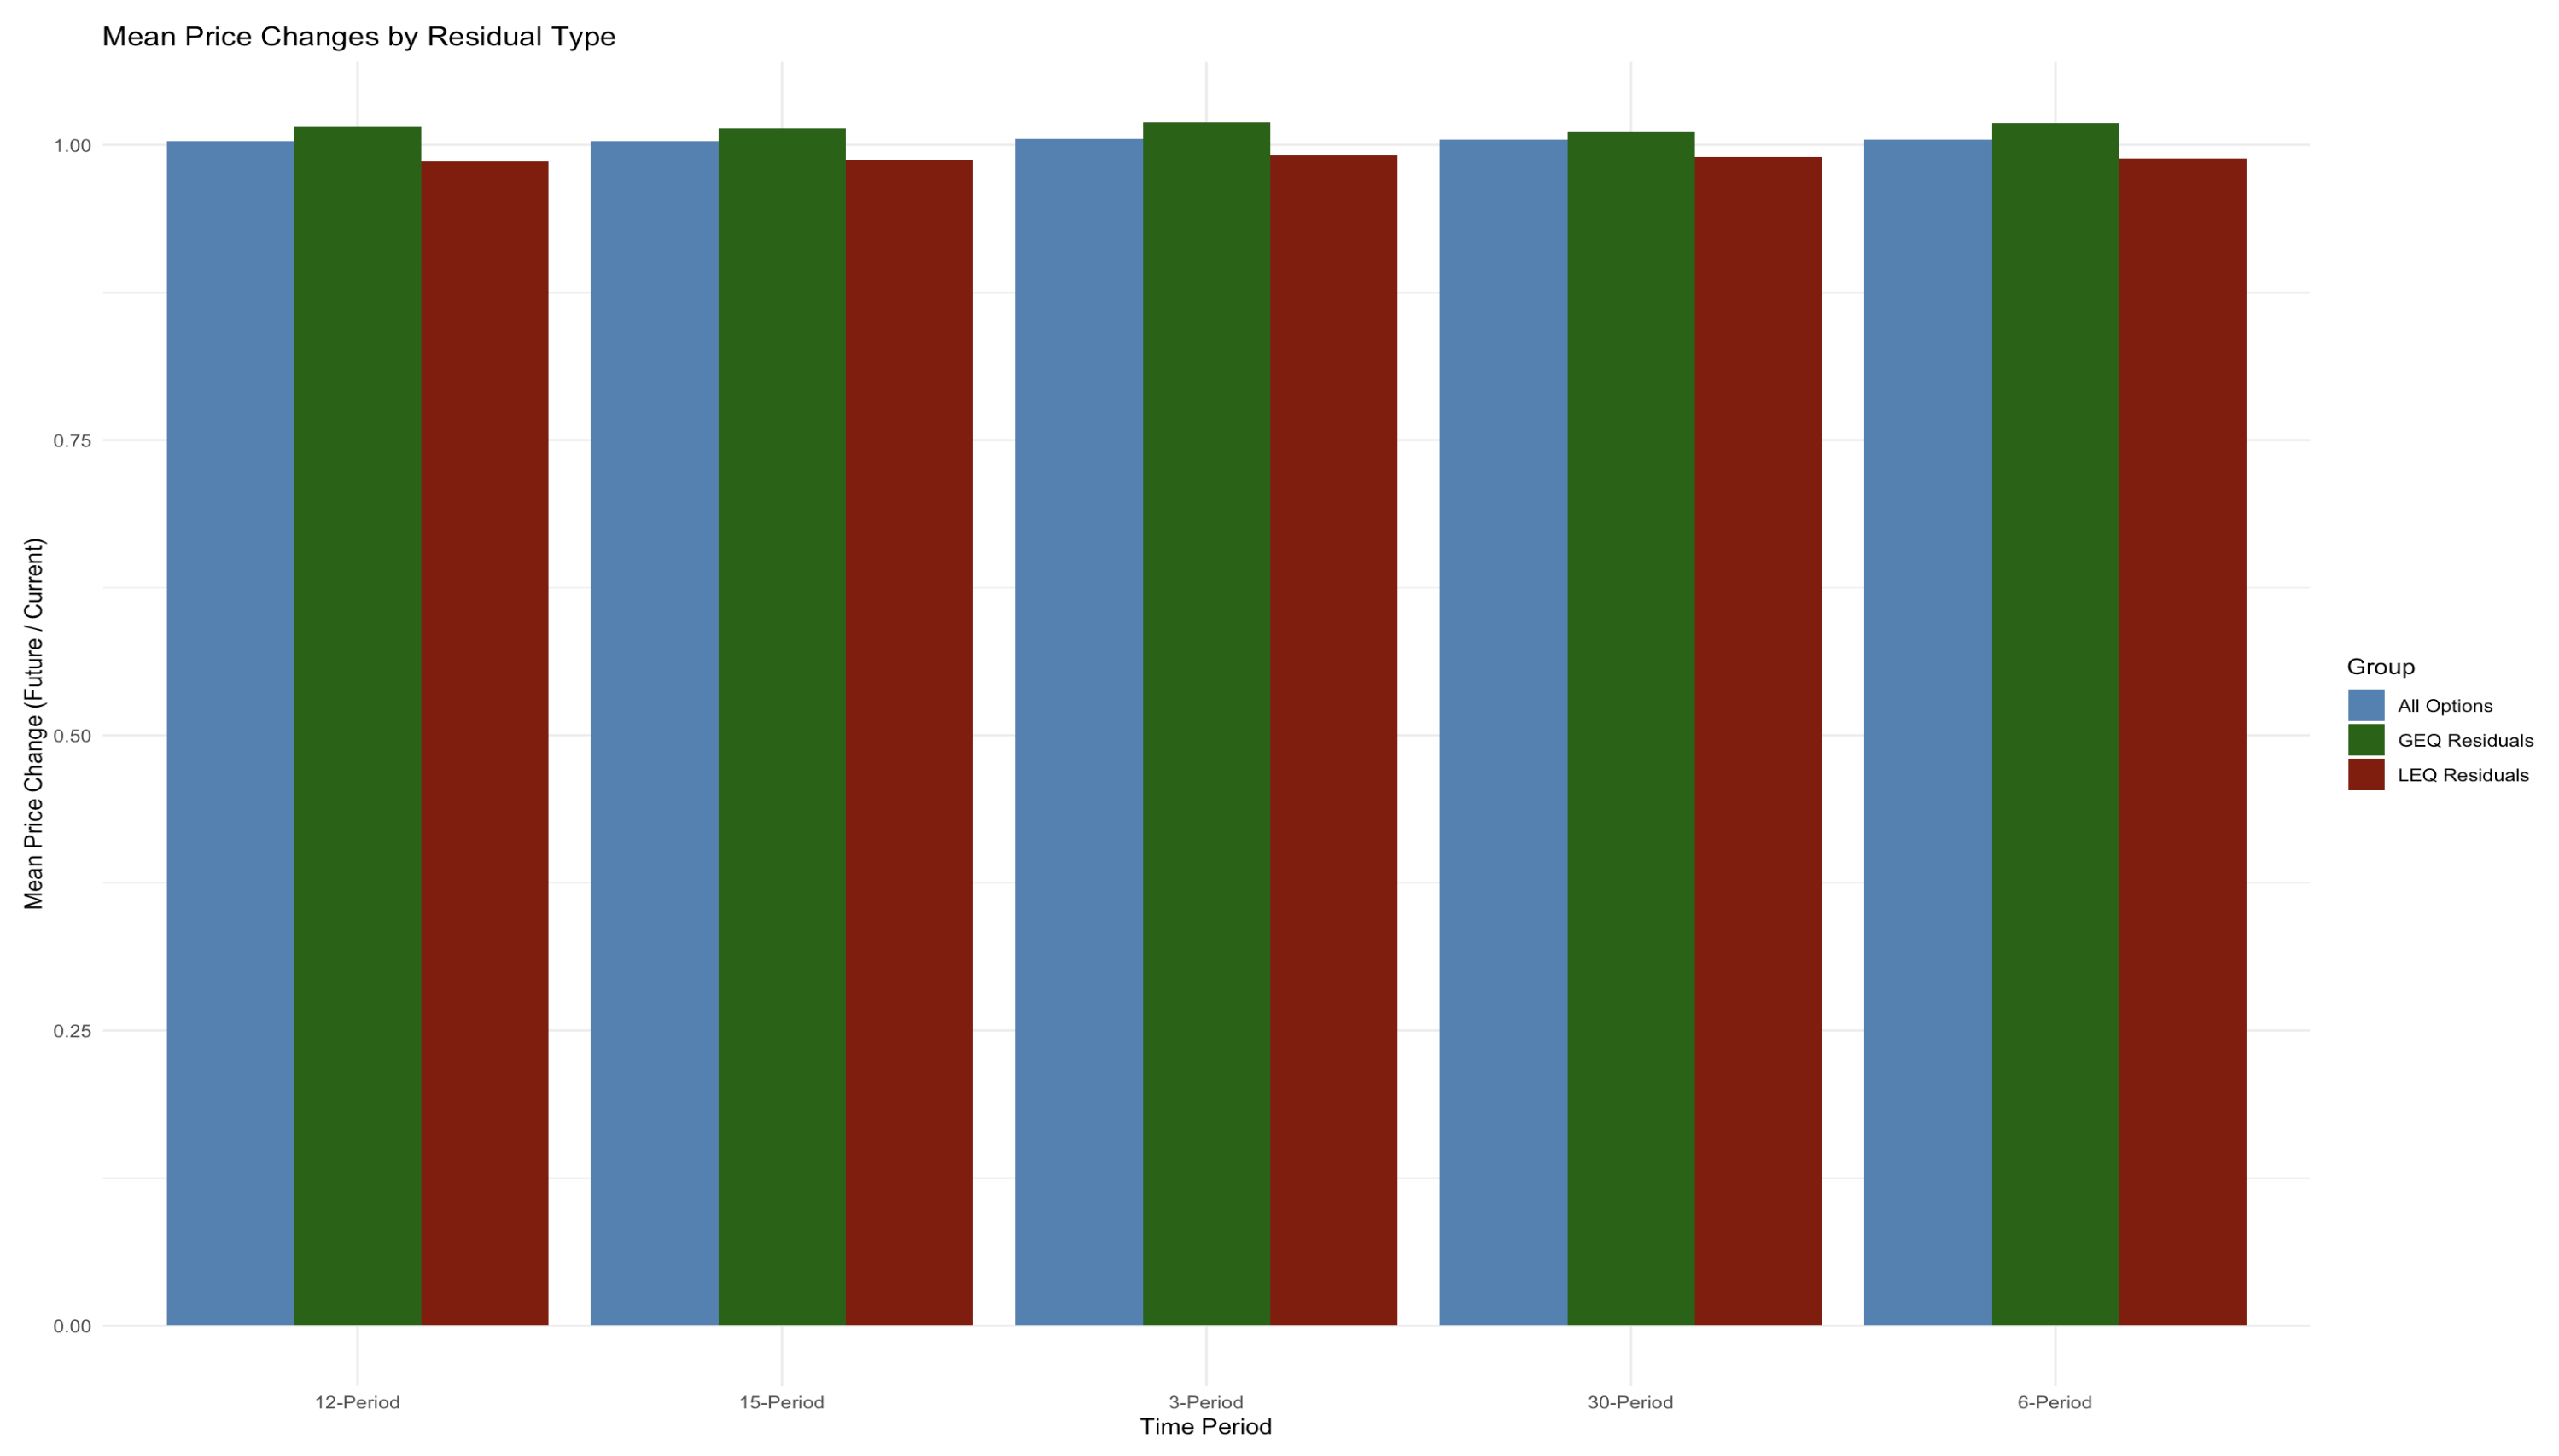
\includegraphics[width=0.8\linewidth]{data/results/mean_price_diff.png}
  \caption{Mean future price ratios by residual group}
  \label{fig:price-diff}
\end{figure}

Figure \ref{fig:price-diff} displays the average future price changes stratified by residual group across different forecast horizons. Options with high residuals (where the model overestimates actual prices) consistently exhibit higher mean price ratios compared to options with low residuals (where the model underestimates actual prices). This pattern supports the directional hypothesis that KNN model residuals contain predictive information for short-term price movements.

\section{Trading Simulation}

\subsection{Signal Generation and Trade Execution}

Trading signals were generated on the test dataset using KNN model predictions. Long positions were initiated when residuals exceeded the 95th percentile threshold $r_t > \bar{r}$, indicating undervalued options. Short positions were initiated when residuals fell below the negative threshold $r_t < -\bar{r}$, indicating overvalued options.

For each trade, the profit or loss was calculated using the future price ratio $price\_diff_x$:
\begin{align*}
\alpha_{\text{long}} &= (price_t \cdot price\_diff_x) - price_t,\\
\alpha_{\text{short}} &= price_t - (price_t \cdot price\_diff_x).
\end{align*}

\subsection{Performance Evaluation}

Based on the hypothesis testing results, we implemented the trading strategy using the 6-period horizon, where the null hypothesis was fully rejected. The strategy executed 5,268 trades and generated \$1,685 in cumulative profit.

\subsection{Statistical Significance Testing}

To assess the statistical significance of our results, we conducted a randomized baseline comparison. We test the null hypothesis:

\[
H_0: \alpha_{\text{strategy}} = \alpha_{\text{random}}
\]

where $\alpha_{\text{strategy}}$ is the cumulative return from our residual-based trading signals and $\alpha_{\text{random}}$ is the expected return from random trading.

For each of 100 Monte Carlo simulations, we randomly selected $N = 5,428$ trades from the test dataset and assigned random long/short positions with equal probability:

\[
\alpha_{\text{random},i} = \begin{cases}
(price_{t,i} \cdot price\_diff_{6,i}) - price_{t,i} & \text{with probability } 0.5 \\
price_{t,i} - (price_{t,i} \cdot price\_diff_{6,i}) & \text{with probability } 0.5
\end{cases}
\]

The cumulative return for each simulation was calculated as $\sum_{i=1}^{N} \alpha_{\text{random},i}$. The empirical null distribution yielded a 95th percentile threshold of \$424.42. Since our observed return of \$2684.96 exceeds this threshold, we reject $H_0$ and conclude that the strategy performs significantly better than random selection at the 5\% significance level.


\section{Empirical Bayes Shrinkage of KNN Residuals}

We reinterpret the residuals from the KNN model as noisy observations of latent mispricings and apply Empirical Bayes shrinkage to improve signal estimation. This builds on the framework of compound decision theory and shrinkage estimation as introduced in Efron (2011) \cite{efron2011tweedie}.

\subsection{Modeling Assumptions}

Assume the following hierarchical model:

\[
r_i \sim \mathcal{N}(\theta_i, \sigma^2), \quad \theta_i \sim g(\theta)
\]

Our objective is to estimate \( \theta_i \), the latent mispricing, using the posterior expectation:

\[
\hat{\theta}_i = \mathbb{E}[\theta_i \mid r_i]
\]

By Tweedie's formula:

\[
\hat{\theta}_i = r_i + \sigma^2 \cdot \frac{d}{dr} \log f(r_i)
\]

where \( f(r) \) is the marginal density of residuals.

\subsection{Shrinkage via Tweedie's Formula}

We estimate \( f(r) \) using kernel density estimation and compute the derivative \( f'(r) \) numerically. The posterior-shrunk mispricing estimate is then:

\[
\hat{\theta}_i = r_i + \sigma^2 \cdot \frac{f'(r_i)}{f(r_i)}
\]

\subsection{Bayesian-Adjusted Trading Strategy}

Let \( \hat{\theta}_i \) be the posterior estimate. Define trade signals based on thresholds derived from the posterior distribution:

\[
\text{Buy if } \hat{\theta}_i > \Phi^{-1}(0.95) \cdot \sigma_\theta, \quad
\text{Sell if } \hat{\theta}_i < \Phi^{-1}(0.05) \cdot \sigma_\theta
\]

Returns are defined by the same formula used in the previous trading simulation.

Total return across all posterior-filtered trades is:

\[
\alpha_{\text{strategy}} = \sum_{i \in T_{\text{long}}} \alpha_{\text{long}, i} + \sum_{j \in T_{\text{short}}} \alpha_{\text{short}, j}
\]

This algorithm executed 340 trades, with a total return of \$742.62. The outcome of this is far more profitable, in terms of dollars per trade, than our previous naive model. Applying shrinkage allows the model to find trades that are more likely to be profitable, at the cost of the number of trades.

\section{Results}

Usually, option contracts cost 0.65\$ per contract in commission fees. For real-time application, this cost structure fundamentally alters the viability of our trading strategies. The original KNN residual-based approach generated \$1,685 profit across 5,268 trades, yielding \$0.32 profit per trade. After accounting for \$0.65 commission per trade, this strategy would result in a net loss of \$1,739.20 (\$1,685 - 5,268 * \$0.65), making it unprofitable in practice.

In contrast, the Empirical Bayes shrinkage method executed only 340 trades while generating \$742.62 in profit, achieving \$2.18 profit per trade. After commission costs of \$221 (340 * \$0.65), the net profit remains positive at \$521.62. This represents a 1550\% improvement in per-trade profitability compared to the original approach.

The shrinkage method's superior performance stems from its ability to filter out weak signals through posterior probability estimation. By shrinking residuals toward zero based on their reliability, the Bayesian approach identifies only the most confident mispricings, dramatically reducing false positives that plagued the original strategy. This selectivity transforms an unprofitable high-frequency approach into a viable low-frequency strategy suitable for real-world implementation. 


\section{Discussion}

The residual-based signals produced consistent return differences in favor of positive and negative residuals. The overvalued short trades yielded significantly lower p-values than the undervalued long trades in Table \ref{tab:mean-return}, suggesting that the model's ability to identify overpriced options may be more reliable than its capacity to detect underpriced ones.

The cross validation in selecting the optimal $k$ used a sequencing function to generate a list of numbers as a function of $n$ where $n$ is the number of rows. However, this was done arbitrarily, to reduce computational overhead. The optimal $k$ could fall outside of this range, and may in fact be 1. The figure below illustrates this fact, showing the residual mean squared error decrease greatly when approaching 1.

\begin{figure}[h]
  \centering
  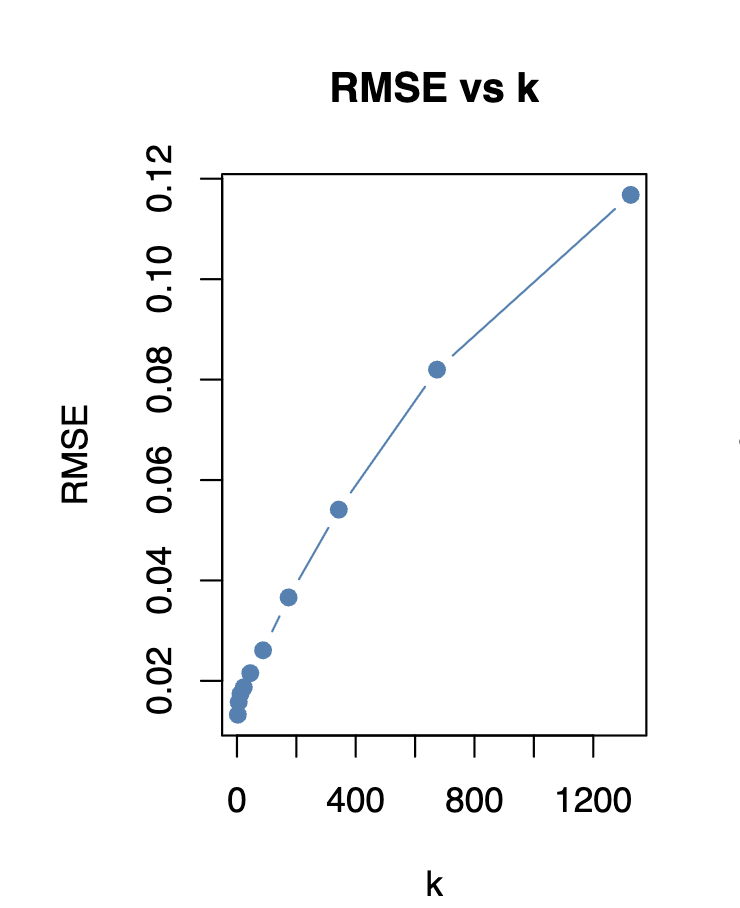
\includegraphics[width=0.8\linewidth]{data/results/knn_rmse.png}
  \caption{KNN RMSE by k value}
  \label{fig:knn-rmse}
\end{figure}

It is possible that Nearest-neighbor interpolation may be the best model fit, however it will lead to a large amount of variance in this model. While nearest-neighbor interpolation (\( k = 1 \)) may offer the best local fit in terms of minimizing bias, it typically results in high variance and overfitting, particularly in noisy or high-dimensional datasets \cite{caruana2006empirical}. For this reason, choosing a $k$ greater than 1 is strongly recommended in non-spatial applications such as financial modeling, where data is not naturally embedded in low-dimensional geometric space.

From a Bayesian perspective, the KNN model can be interpreted as providing a data-driven prior distribution for option prices conditional on the selected Greeks. The residuals $r_t = \hat{y}_t - y_t$ represent deviations from this prior, effectively capturing information not encoded in the feature set. When these residuals exhibit predictive power for future price movements, they suggest that the market has not fully incorporated all available information into current prices, creating exploitable inefficiencies.

The posterior belief about an option's true value can be viewed as a combination of the KNN prior estimate and the residual information. Options with large positive residuals (where $\hat{y}_t > y_t$) indicate that the model's prior suggests higher value than the market price, potentially signaling undervaluation. Conversely, large negative residuals suggest overvaluation relative to the model's expectations.

While the profits observed in backtesting were modest, the approach performed significantly better than random trading according to the null threshold. However, we assume zero execution friction; incorporating slippage and fees is a promising direction for future refinement. Though for this analysis, KNN served as an effective non-parametric estimator for the conditional distribution of standardized option prices given \verb|delta|, \verb|gamma|, \verb|moneyness|, and \verb|rho|, more sophisticated models such as random forests and boosted trees could potentially capture additional nonlinear relationships \cite{caruana2006empirical}.

To better understand the drivers of trade success, we conducted K-means clustering on executed trades using key predictive features: \verb|delta|, \verb|gamma|, \verb|moneyness|, and \verb|rho|. 

A Chi-squared test was conducted to determine if $P(\text{Profit} | \text{Cluster}) \neq P(\text{Profit})$ at $p=0.05$. This analysis revealed structurally distinct trade clusters with significantly different profit probabilities, particularly among short-sell trades. The following figure shows the 10 clusters created, by profitability.

\begin{figure}[h]
  \centering
  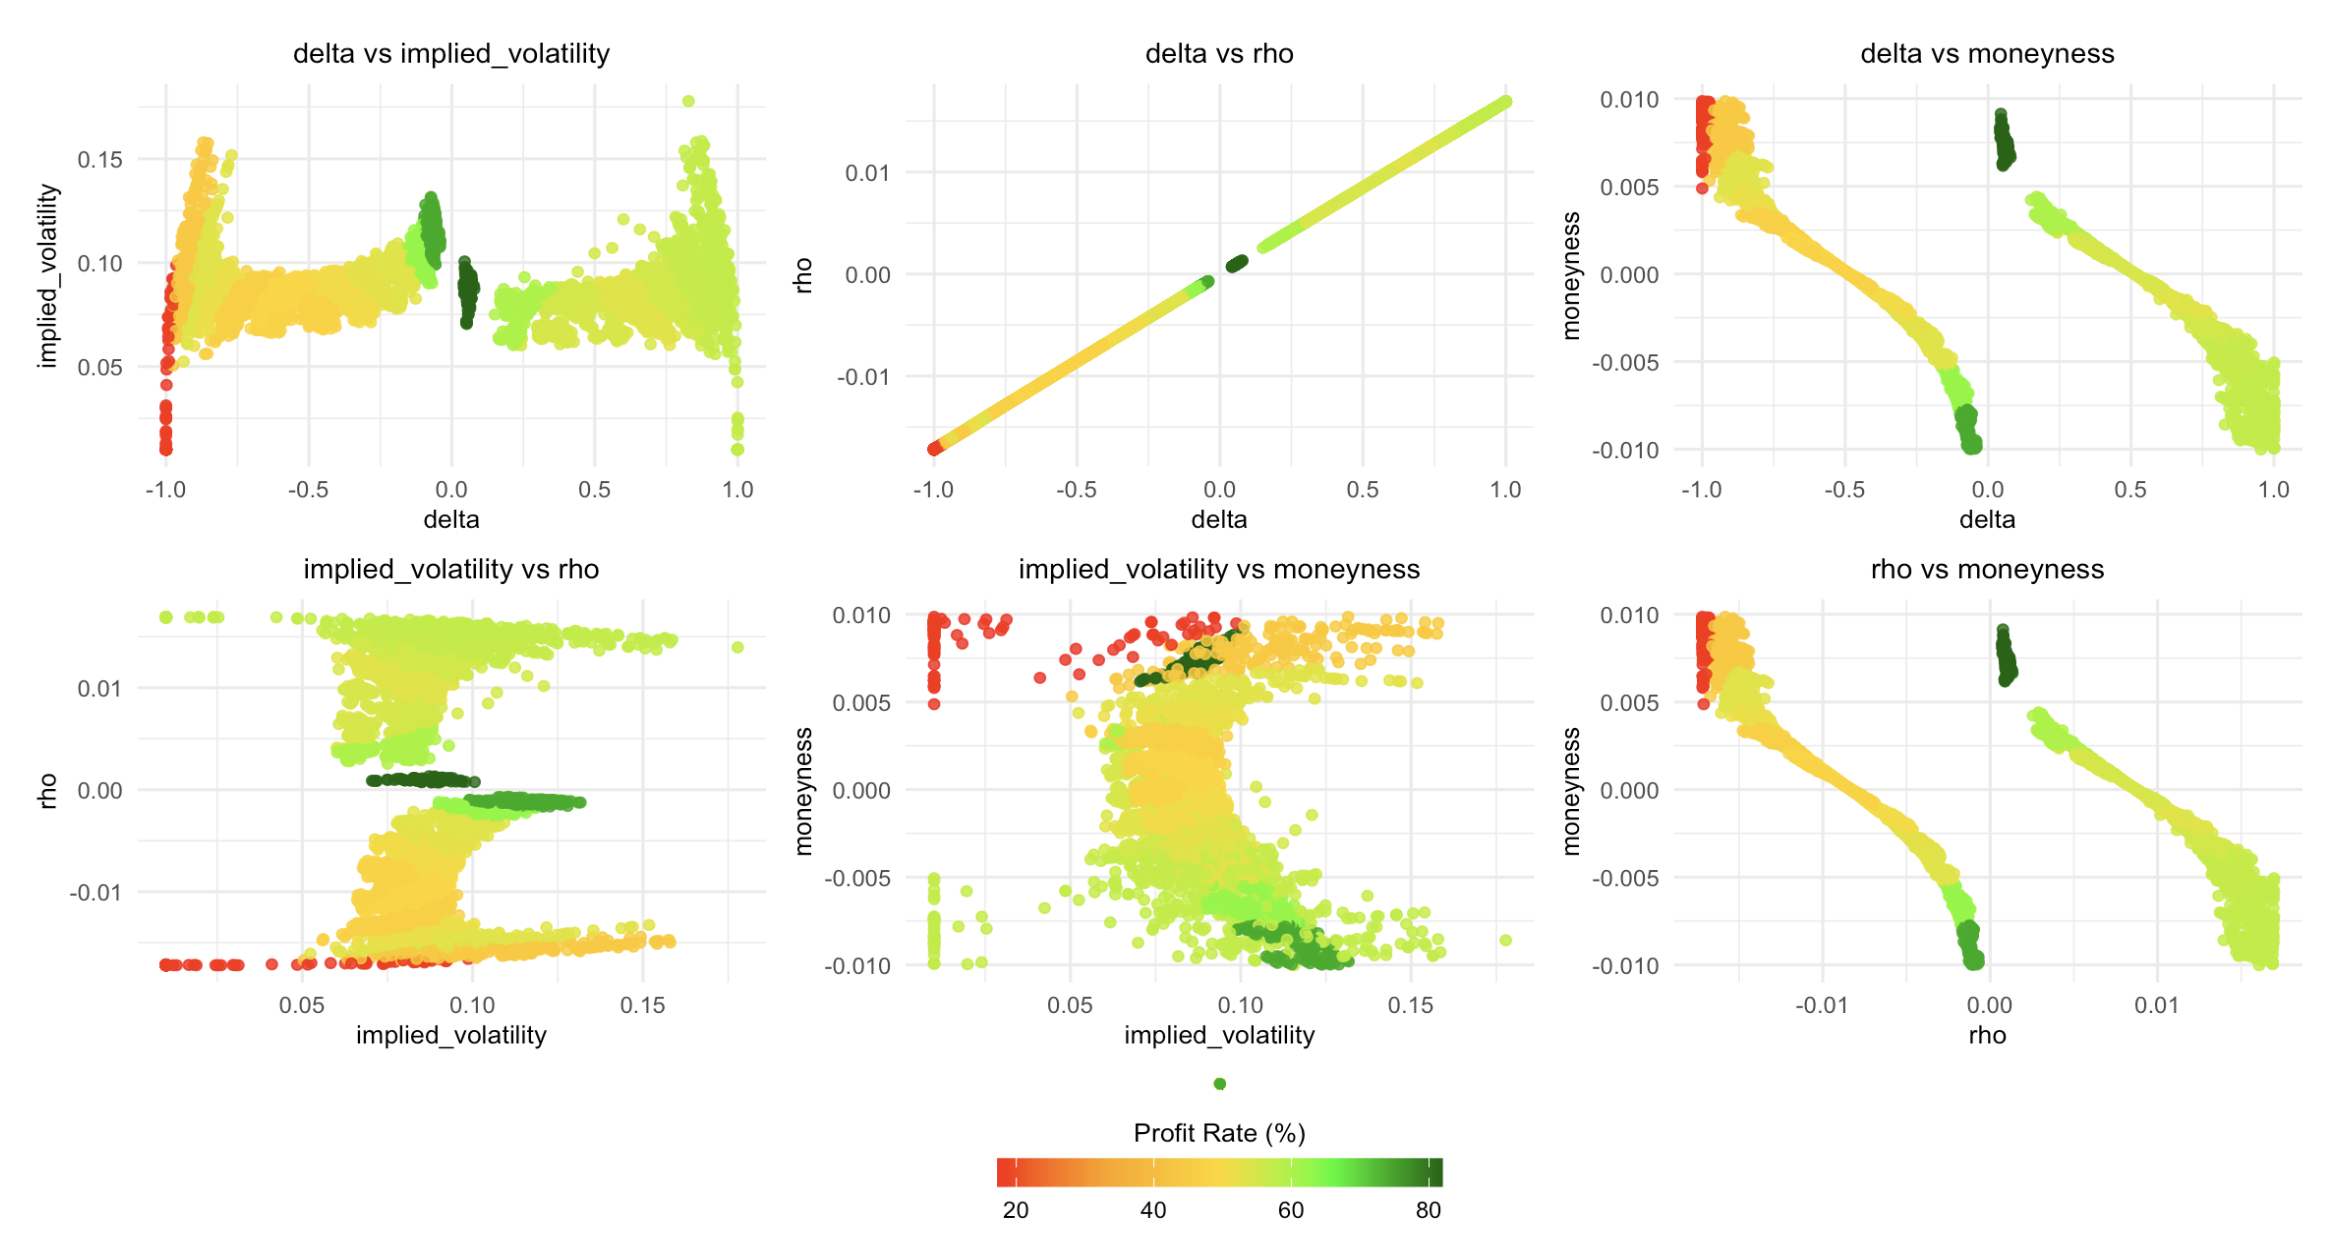
\includegraphics[width=1\linewidth]{data/results/clusters.png}
  \caption{Clusters by profitability}
  \label{fig:clusters}
\end{figure}

This figure shows us the trends in our data, such as OTM puts being particularly profitable. These clusters can help us identify areas of weakness, and add an additional layer of robustness to our trade execution. This can be done with the help of a rule engine, which only allows trades within the most profitable clusters.

\begin{figure}[h]
  \centering
  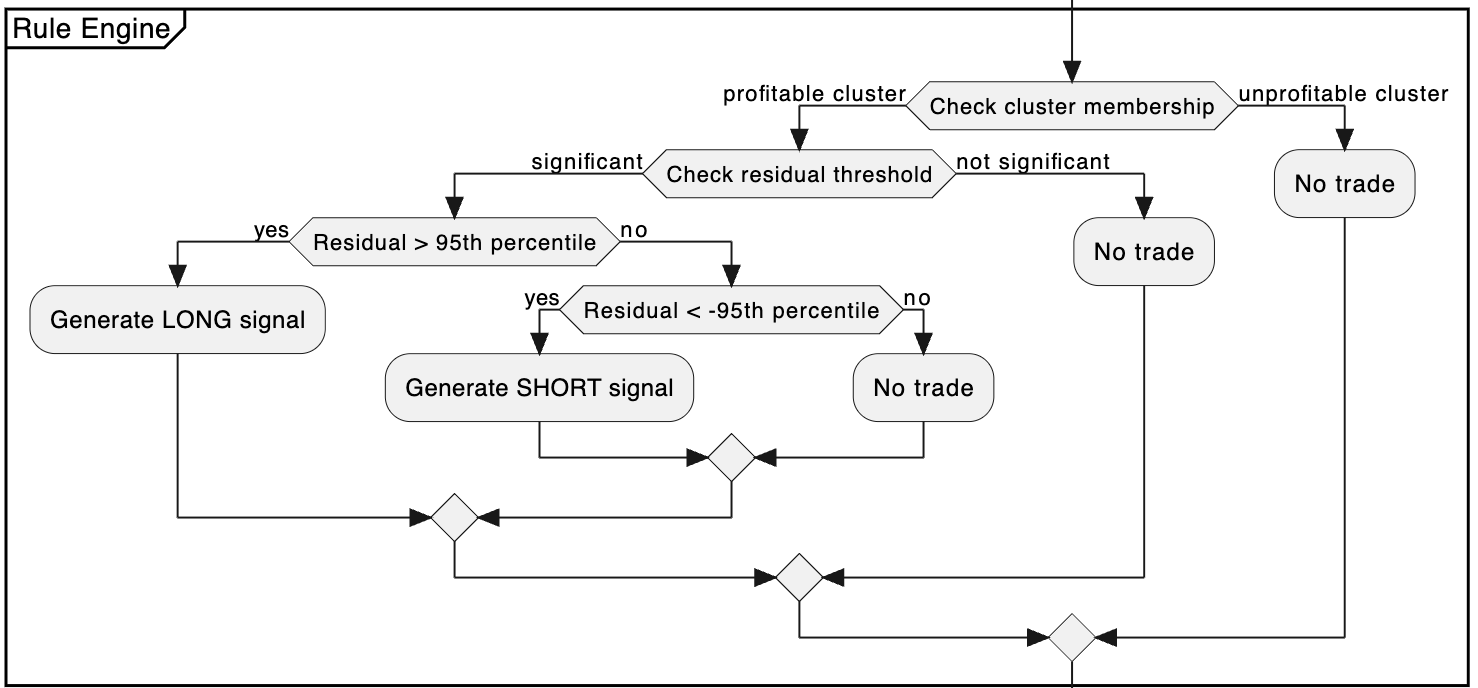
\includegraphics[width=0.8\linewidth]{data/results/algo.png}
  \caption{Rules to execute trade}
  \label{fig:algo}
\end{figure}

\section{Conclusion}

This paper introduces a residual-driven K-Nearest Neighbors framework for detecting and exploiting short-term mispricings in equity options. By predicting standardized option prices using a carefully selected subset of option Greeks, we demonstrate that the residuals from the KNN model carry directional information about future price movements. Through hypothesis testing , we identify statistically significant deviations in residuals that serve as actionable trading signals.

A trading strategy built on these residual-based signals achieves performance that significantly exceeds a randomized baseline, generating over \$2 per trade in profit across hundreds of trades and surpassing the empirical 95th percentile of the Monte Carlo simulated outcomes. This finding underscores the presence of persistent inefficiencies in the short-term options market that can be captured using non-parametric techniques with minimal assumptions.

Beyond its practical implications, our framework showcases how interpretable machine learning models can be fused with financial domain knowledge to produce both profitable and statistically sound trading strategies. Future work may extend this framework by incorporating Bayesian uncertainty estimation, dynamic $k$ selection, or hybrid ensemble models. Additionally, analyzing how residual signals evolve over intraday time segments could further enhance signal quality and timing.

Conclusively, the approach outlined here represents a potentially scalable, data-driven methodology that bridges predictive modeling with hypothesis-driven market interpretation—offering both theoretical insight and empirical edge.

\section{References}
\bibliographystyle{plain}
\bibliography{refs}

\appendix
\section{Black-Scholes Formulas}
\subsection{Option Pricing Formulas}
The Black-Scholes model for European option pricing is given by the following formulas:

\subsubsection{Call Option Price}
\begin{equation}
C(S, K, T, r, \sigma) = S \cdot N(d_1) - K e^{-rT} \cdot N(d_2)
\end{equation}

\subsubsection{Put Option Price}
\begin{equation}
P(S, K, T, r, \sigma) = K e^{-rT} \cdot N(-d_2) - S \cdot N(-d_1)
\end{equation}

\subsubsection{Parameters $d_1$ and $d_2$}
\begin{equation}
d_1 = \frac{\ln(S/K) + (r + \sigma^2/2)T}{\sigma\sqrt{T}}
\end{equation}

\begin{equation}
d_2 = d_1 - \sigma\sqrt{T}
\end{equation}

where:
\begin{itemize}
  \item $S$ = Current stock price
  \item $K$ = Strike price
  \item $T$ = Time to expiration (in years)
  \item $r$ = Risk-free interest rate
  \item $\sigma$ = Volatility of the underlying asset
  \item $N(\cdot)$ = Cumulative distribution function of the standard normal distribution
\end{itemize}

\subsection{Option Greeks}
The Greeks measure the sensitivity of option prices to various factors:

\subsubsection{Delta}
Measures the rate of change of option price with respect to changes in the underlying asset's price.

\textbf{Call Option Delta:}
\begin{equation}
\Delta_{call} = N(d_1)
\end{equation}

\textbf{Put Option Delta:}
\begin{equation}
\Delta_{put} = N(d_1) - 1
\end{equation}

\subsubsection{Gamma}
Measures the rate of change of delta with respect to changes in the underlying price.
\begin{equation}
\Gamma = \frac{N'(d_1)}{S\sigma\sqrt{T}} = \frac{e^{-\frac{d_1^2}{2}}}{S\sigma\sqrt{2\pi T}}
\end{equation}

Gamma is the same for both call and put options.

\subsubsection{Theta}
Measures the rate of change of option price with respect to the passage of time (time decay).

\textbf{Call Option Theta:}
\begin{equation}
\Theta_{call} = -\frac{S N'(d_1)\sigma}{2\sqrt{T}} - rKe^{-rT}N(d_2)
\end{equation}

\textbf{Put Option Theta:}
\begin{equation}
\Theta_{put} = -\frac{S N'(d_1)\sigma}{2\sqrt{T}} + rKe^{-rT}N(-d_2)
\end{equation}

Theta is typically expressed in value per day, dividing by 365.

\subsubsection{Vega}
Measures the rate of change of option price with respect to changes in volatility.
\begin{equation}
Vega = S\sqrt{T}N'(d_1)
\end{equation}

Vega is the same for both call and put options and is typically expressed as change per 1\% change in volatility.

\subsubsection{Rho}
Measures the rate of change of option price with respect to changes in the risk-free interest rate.

\textbf{Call Option Rho:}
\begin{equation}
\rho_{call} = KTe^{-rT}N(d_2)
\end{equation}

\textbf{Put Option Rho:}
\begin{equation}
\rho_{put} = -KTe^{-rT}N(-d_2)
\end{equation}

Rho is typically expressed as change per 1\% change in interest rate.

\subsection{Implied Volatility}
Implied volatility is the volatility value that, when input into the Black-Scholes formula, yields a theoretical option price equal to the market price. It is typically solved using numerical methods such as the Newton-Raphson method:

\begin{equation}
\sigma_{n+1} = \sigma_n - \frac{BS(S, K, T, r, \sigma_n) - Market\_Price}{Vega}
\end{equation}

where $BS(\cdot)$ is the Black-Scholes pricing function and iterations continue until convergence.

\subsection{Put-Call Parity}
For European options on non-dividend paying stocks:
\begin{equation}
C + Ke^{-rT} = P + S
\end{equation}

This relationship can be used to derive the price of a put option from a call option with the same strike and expiration, or vice versa.

\end{document}